\section{Background and Problem}

\begin{frame}
	\frametitle{Planning under Uncertainty}
	\framesubtitle{Domain Characteristics}
	
	\begin{columns}[T]
		\begin{column}{.7\textwidth}
			\begin{itemize}
				\item<2-> A system is controlled by one or more \textit{agents}
				\item<3-> \textit{Uncertain domain dynamics}, i.e.\\ uncertainty may be present in:
				\begin{itemize}
					\item Execution of actions (e.g., robot may slip)
					\item Exogenous factors (e.g., doors open/closed)
					\item Percepts (e.g., sensor noise)
				\end{itemize}
				\item<4-> \textit{Sequential decision making}
				\begin{itemize}
					\item Non-myopic agents
					\item Selection of actions with high future pay-off
				\end{itemize}
			\end{itemize}
		\end{column}
		\begin{column}{.35\textwidth}
		%	%\vspace{-30pt}
			\includegraphics[width=1.0\textwidth, right]{figures/path-planning2}
		\end{column}
	\end{columns}
\end{frame}

\begin{frame}
	\frametitle{Planning under Uncertainty}
	\framesubtitle{Example Domains}
	
	\begin{columns}[t]
		\begin{column}{.3\textwidth}
			\centering 
			\begin{overlayarea}{\linewidth}{4.75cm}
				\includegraphics[width=\columnwidth]{figures/path-planning}
			\end{overlayarea}
			\captionof*{figure}{\scriptsize\textit{\textcolor{tudBlack}{Path planning}} \cite{hawes2017strands, iocchi2016practical}}
		\end{column}
		\begin{column}{.25\textwidth}
			\centering
			\begin{overlayarea}{\linewidth}{4.75cm}
				\centering
				\vspace{-18pt}
				\includegraphics[width=0.75\columnwidth]{figures/motion-planning}\\
				{\scriptsize\textit{Motion planning}}\\\vspace{6pt}
				\includegraphics[width=0.85\columnwidth]{figures/dialog_system_2}
			\end{overlayarea}
			\captionof*{figure}{\scriptsize\textit{\textcolor{tudBlack}{Dialog Management}} \cite{chinaei2011}}
		\end{column}
		\begin{column}{.3\textwidth}
			\centering
			\begin{overlayarea}{\linewidth}{4.75cm}
				\vspace{0pt}
				\includegraphics[width=\columnwidth]{figures/operations-planning5}
			\end{overlayarea}
			\captionof*{figure}{\scriptsize\textit{\textcolor{tudBlack}{Operations planning}} \cite{aberdeen2004decision, sigaud2010}}
		\end{column}
	\end{columns}
	\imgsrc*[Image credits]{Hawes et al. \cite{hawes2017strands}, \href{https://coaches.greyc.fr}{Iocchi et al.} \cite{iocchi2016practical}, \href{http://www.coppeliarobotics.com/helpFiles/en/motionPlanningModule.htm}{V-REP Manual}, Bemidji State University}
\end{frame}
% Examples Operations Planning:
% - Military Operations Planning: Decision-Theoretic Military Operations Planning
% - Markov Decision Processes in AI: (Operations Planning Rover Exploration) https://www.safaribooksonline.com/library/view/markov-decision-processes/9781118620106/xhtml/Chapter15.html
% - Project Management: Engineering the Decision-Making Process Using Multiple Markov Theories and DEMO
\imgsrc*{off}

\begin{frame}
	\frametitle{Planning under Uncertainty}
	\framesubtitle{Typical Development Routine}
	\centering
	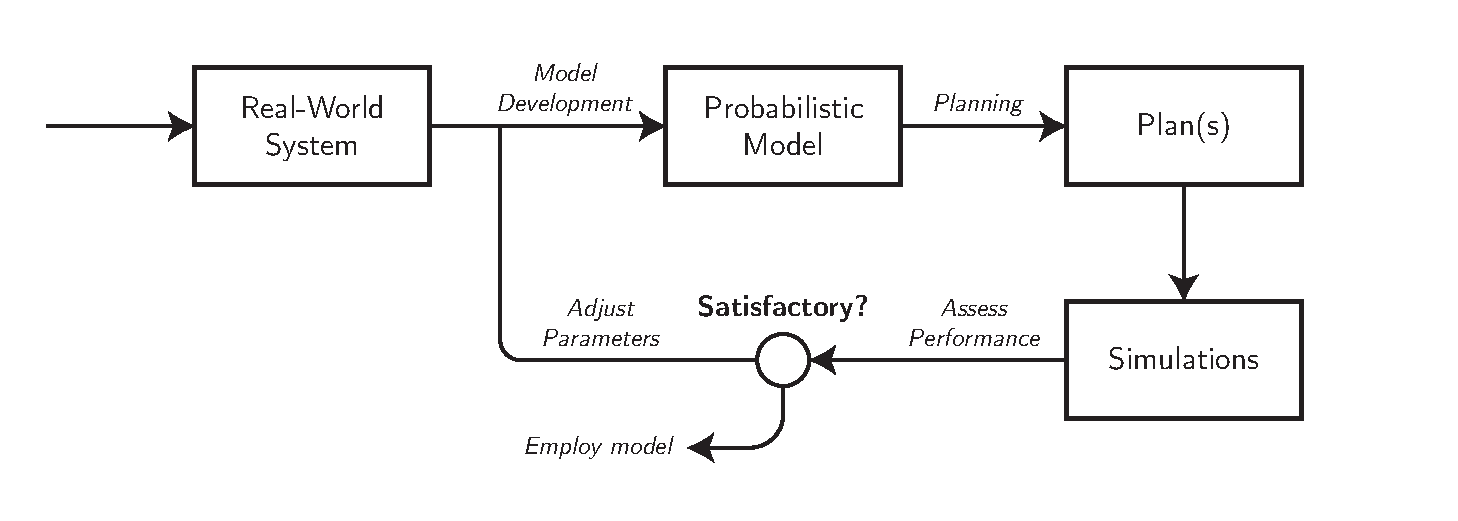
\includegraphics[width=\textwidth]{figures/high-level-planning-diagram}
\end{frame}

\begin{frame}
	\frametitle{Planning under Uncertainty}
	\framesubtitle{Markov Decision Processes (MDPs)}
	
	In DTP systems are modeled by probabilistic models, e.g. MDPs:
	\begin{columns}[T]
		\begin{column}{0.6\textwidth}
			\begin{definition}
				An MDP is a 5-tuple $\mathcal{M} = (\mathcal{S}, s_0, A, \delta, R)$:
				\begin{itemize}
					\item $\mathcal{S}$ is the state-space, $s_0 \in \mathcal{S}$ the initial state
					\item $A$ is the action-space
					\item $\delta: \mathcal{S} \times A \times \mathcal{S} \mapsto [0, 1]$ is the transition function % $\delta: S \times S \times A \mapsto [0,1]$
					\item $R: \mathcal{S} \times A \times \mathcal{S} \mapsto \mathbb{R}$ is the reward function
				\end{itemize}
			\end{definition}
		\end{column}
		\begin{column}{0.425\textwidth}
			\vspace{26pt}
			\includegraphics[width=\linewidth]{figures/mdp-2v3}
		\end{column}
	\end{columns}
\end{frame}

\begin{frame}
	\frametitle{Planning under Uncertainty}
	\framesubtitle{Planning with MDPs}
	\vspace{-10pt}
	\begin{center}
		\includegraphics<1|handout:0>[width=0.9\textwidth]{figures/planning_routine/mdp-planning-diagram-v2-1}
		\includegraphics<2|handout:0>[width=0.9\textwidth]{figures/planning_routine/mdp-planning-diagram-v3-2}
		\includegraphics<3|handout:0>[width=0.9\textwidth]{figures/planning_routine/mdp-planning-diagram-v3-3}
		\includegraphics<4|handout:0>[width=0.9\textwidth]{figures/planning_routine/mdp-planning-diagram-v3-4}
		\includegraphics<5>[width=0.9\textwidth]{figures/planning_routine/mdp-planning-diagram-v3-5}
	\end{center}
\end{frame}

\begin{frame}
	\frametitle{Planning under Uncertainty}
	\framesubtitle{Model Development}
	
	\textcolor{tudBlack}{\textbf{Problem:}} How to obtain a suitable MDP for offline planning?
	\pause
	\vfill
	\textcolor{tudBlack}{\textbf{Classical approach:}} Model development by a \textit{human designer}, however:
	\begin{itemize}
		\item Requires significant effort (e.g., trial-and-error)
		\item Typically demands knowledge/experience, accompanied by high costs
	\end{itemize}
	\pause
	\vfill
	\textcolor{tudBlack}{\textbf{Alternative:}} Use Reinforcement Learning instead of Planning, however:
	\begin{itemize}
		\item Requires direct interaction with environment %(slow in complex dynamic environment) % (chance of errors)
		\item One might require \textit{reusable} models, applicable for multiple tasks % You do have model-based RL, but we might want a model that generalizes for multiple tasks
		%\item Still requires definition of state-spaces (and actions and rewards)
	\end{itemize}
\end{frame}

\begin{frame}[t]
	\frametitle{Planning under Uncertainty}
	\framesubtitle{Model Development}
	\vspace{8pt}
	\textcolor{tudBlack}{\textbf{Problem:}} How to obtain a suitable MDP for offline planning?\\
	\vspace{14pt}
	\textcolor{tudblue}{\textbf{Idea:}} Automate the development process through~learning~algorithms 
	\begin{itemize}
		\item<2-> Making use of a dataset describing the system's dynamics
		\item<3-> Learn the components of MDPs:
		\begin{itemize}
			\item State space (e.g., clustering, time-state merging)
			\item Transition probabilities (e.g., maximum likelihood, Bayesian inference)
			\item \semitransp[40]{Emission probabilities in POMDPs (e.g., Baum-Welch, gradient ascent)}
		\end{itemize}
	\end{itemize}
	\vspace{10pt}
	\onslide<4->{\textcolor{tudBlack}{\textit{Next Question:} How to set the hyperparameters for these algorithms?}}
\end{frame}

% !! Translating our earlier question into research questions !!

%\setbeamercovered{transparent}

\begin{frame}[t]
\frametitle{Problem Description}
\framesubtitle{Research Questions [1/2]}

\begin{block}{Main Research Question}<2->
%	How can the task of learning a \textit{performance-maximizing} MDP from a dataset be automated?
How can the task of obtaining a (discrete) MDP that maximizes the yielded performance of executing plans that are derived from it, given a dataset about the system under consideration, be automated?
\end{block}

\begin{description}
	\item<3->[RQ1] Which \textcolor{tudOrange}{learning algorithms} exist that can be employed for learning MDPs from data for systems involving uncertainty that require plans for automated control?
	\item<4->[RQ2] How should a  \textcolor{tudOrange}{performance measure} be defined which can be used to fairly compare the value of different MDPs?
\end{description}

\end{frame}

\begin{frame}[t]
	\frametitle{Problem Description}
	\framesubtitle{Research Questions [2/2]}
	
	\begin{block}{Main Research Question}
		%	How can the task of learning a \textit{performance-maximizing} MDP from a dataset be automated?
		How can the task of obtaining a (discrete) MDP that maximizes the yielded performance of executing plans that are derived from it, given a dataset about the system under consideration, be automated?
	\end{block}
	
	\begin{description}
		\item<1->[RQ3] How can the  \textcolor{tudOrange}{parameter space} of model learning algorithms  \textcolor{tudOrange}{cost-effectively be explored} towards a global maximizer with only limited knowledge about the system under consideration?
		\item<2->[RQ4] How can the hierarchy of \textcolor{tudOrange}{different abstraction levels} be exploited to find a performance-maximizing MDP in a more cost-effective way?
	\end{description}
	
\end{frame}

%\setbeamercovered{invisible}

\begin{frame}
	\frametitle{Problem Description}
	\framesubtitle{Problem Statement}
	
	\begin{block}{Problem Statement}
	Given \textcolor{tudblue}{a set $E$ of execution traces} describing the dynamics of a system that involves uncertainty, \onslide<2->{an MDP $\mathcal{M}$ needs to be developed, utilizing \textcolor{tudblue}{learning algorithms parameterized by a set of hyperparameters $\theta$}}\onslide<3->{ configured in such way to \textcolor{tudblue}{maximize the performance yielded} by following the policies computed from this model in a real-world setting.}
	\end{block}
	
\end{frame}

\begin{frame}
	\frametitle{Problem Description}
	\framesubtitle{Related Work}
	
	\begin{itemize}
		\item<2-> Model Learning Algorithms
		\begin{itemize}
			\item Baum-Welch for HMMs/POMDPs \cite{welch2003hidden}, e.g., Shatkay et al. \cite{shatkay1997}
			\item Best-First Model Merging
			\item State-Merging by Trajectory Clustering \cite{nikovski2000learning}
		\end{itemize}
		\item<3-> Reinforcement Learning
		\begin{itemize}
			\item Model-based RL and Integrated Architectures, e.g. DYNA \cite{guez2012efficient}
			\item Active RL \cite{epshteyn2008active} - Uses provided MDP as blueprint for exploration
			\item \begin{labeling}{Bayesian RL [xx] - }
				\item[Bayesian RL \cite{Poupart2010} -] Resolves exploration-exploitation dilemma by planning in the belief space
			\end{labeling}
		\end{itemize}
		\item<4-> MDPs with Transition Probability Uncertainty
		\begin{itemize}
			\item MDP-IPs \cite{delgado2011efficient}
			\item BMDPs \cite{givan2000bounded}
		\end{itemize}
	\end{itemize}
	
\end{frame}